\documentclass[11pt]{exam}
\input{../Header/packages.sty}
\input{../Header/styleExam.sty}
\input{../Header/mathexpressions.sty}
\input{../Header/headerExam.sty}
\graphicspath{{Algebra/data-algebra/},{Geometrie/data-geometrie/},{Analysis/data-analysis/}} % Setzt den Pfad zu den Bilder fest
%=========================================================
\newcommand{\theme}{Differential- \& Integralrechnung}
\newcommand{\teacher}{Jonas Guler}
\newcommand{\class}{4NaPa}
\renewcommand{\date}{30.10.26}
%=========================================================
\begin{document}
\fontsize{14}{14}\selectfont
%========================================================
\noindent
\begingroup
\renewcommand{\arraystretch}{1.5}
\begin{tabular*}{\textwidth}{l @{\extracolsep{6pt}}l @{\extracolsep{\fill}}l @{\extracolsep{6pt}}l}
	\multicolumn{2}{l}{{\bf \theme}} & {\bf Note:} & {\answerbox}\\
	\multicolumn{2}{l}{{\bf \teacher}} & & \\
	{\bf Klasse:} & {\class} &  {\bf Name:} & {\rule{5cm}{0.5pt}}\\
	{\bf Dauer:} & $45$ Minuten & {\bf Datum:} & {\date}\\[8pt]
\end{tabular*}
\endgroup
\rule[1ex]{\textwidth}{1pt}
%=========================================================
\begin{center}
	\textbf{Bewertungstabelle}\\
	\small Wird von der Lehrperson ausgefüllt\\
	\vspace{5pt}
	\addpoints
	\gradetable[h][questions]\\
	\vspace{5pt}
	Der Rechenweg muss \textbf{vollständig und nachvollziehbar} sein.\\
	Lösen Sie die Prüfung mit einen schwarzen oder blauen Kugelschreiber.\\
	%Als Hilfsmittel ist der Taschenrechner (TI - Nspire CX-II CAS) erlaubt.
	Als Hilfsmittel ist der kleine Taschenrechner (TI-30X o.ä.) und das Formelbüchlein erlaubt.
\end{center}
\rule[1ex]{\textwidth}{1pt}

\vspace{10cm}
\begin{center}
	%\Huge{Repetitionsprüfung}
\end{center}

\newpage
\begin{questions}
%=========================================================
%------------------------TESTFRAGEN
%=========================================================
\question[2]
Bestimme die erste Ableitung der folgenden Funktion schrittweise von Hand. Gib in deinem Lösungsweg an, welche Ableitungsregeln verwendet werden. Die Resultate müssen \textbf{nicht} vereinfacht werden. \[f(x)=3\*\exp{x^2-3x}-6\*\ln{\frac{1}{3}x}\]
\antwort{6}

\noaddpoints
\question[\totalpoints]
\addpoints
Gegeben sind zwei verkettete Funktionen $g_1$ und $g_2$, die wie folgt zusammengesetzt werden: $g_1(x)=\frac{u(x)}{3}+21$ mit $u(x)=3x-63$ und $g_2(x)=2-\frac{1}{v(x)}$ mit $v(x)=\frac{1}{2-x}$.
\begin{parts}
	\part[2] Bestimme durch Anwendung der Kettenregel die beiden Ableitungen $\frac{\d{}}{\d{x}}\,g_1(x)$ und $\frac{\d{}}{\d{x}}\,g_2(x)$.
	\part[2] Zeige, dass $g_1(x)$ und $g_2(x)$ die gleiche Funktionen darstellen.
\end{parts}
\antwort{10}


%---------------------------------------------------------
\newpage
\noaddpoints
\question[\totalpoints]
\addpoints
\begin{parts}
	\part[2] Ergänze und begründe kurz:
	\begin{align*}
		&\int_a^a f(x)\d{x} = \gap{5}\hspace{5cm}\\
		&\int_b^a f(x)\d{x} = \gap{5}
	\end{align*}
\end{parts}
\antwort{4.5}
\begin{solution}
	$\int_a^a f(x)\,\mathrm{d}x = 0$, da die Breite der Rechtecke $0$ ist.\\
	$\int_b^a f(x)\,\mathrm{d}x = -\int_a^b f(x)\,\mathrm{d}x$, da die Breite der Rechtecke negativ wird.
\end{solution}
\begin{parts}
	\setcounter{partno}{1}
	\part[4] Bestimme die folgenden unbestimmten Integrale:
	\begin{enumerate}[label=\roman*)]
		\item $\ds\int \left(5x^4 - 6x^2 + 2\right)\d{x}$
		\item $\ds\int \left(3\*\exp{x} + 4\sin{x}\right)\d{x}$
	\end{enumerate}
\end{parts}
\antwort{13}
\begin{solution}
	\begin{enumerate}[label=\roman*)]
		\item $x^5 - 2x^3 + 2x + c$
		\item $3\,\mathrm{e}^x - 4\cos(x) + c$
		\item $2\ln(x) + \frac{2}{3}x^{\frac{3}{2}} + c$
	\end{enumerate}
\end{solution}


%---------------------------------------------------------
\newpage
\noaddpoints
\question[\totalpoints]
\addpoints
Gegeben ist die Funktion $f(x) = 3 - \frac{1}{3}x^2$ im Intervall $[0,2]$.
\begin{parts}
	\part[2] Skizziere den Graphen von $f$. Zeichne darin die Rechtecke der Obersumme für $n = 6$ ein und begründe, auf welcher Seite du die Höhen abliest.
\end{parts}
\begin{figure}[H]
	\centering
	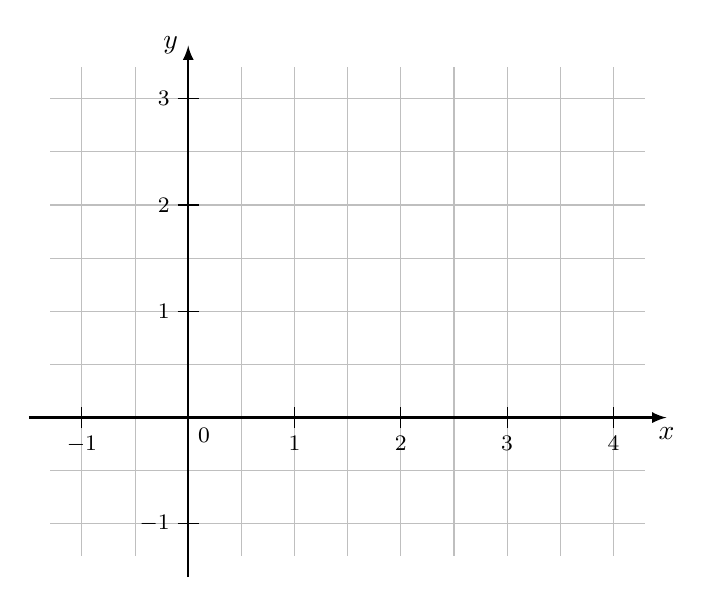
\begin{tikzpicture}[cross/.style={draw, cross out, minimum size=2*(#1-1pt), inner sep=0pt, outer sep=0pt}, x=15mm, y=15mm,
		>=latex,   %Voreinstellung für Pfeilspitzen
		font= \footnotesize, scale=0.9]
		%Raster zeichnen
		\draw [color=gray!50]  [step=7.5mm] (-1.3,-1.3) grid (4.3,3.3);
		% Achsen zeichnen
		\draw[->,thick] (-1.5,0) -- (4.5,0) node[right, below] {\normalsize $x$};
		\draw[->,thick] (0,-1.5) -- (0,3.5) node[above, left] {\normalsize $y$};
		% Achsen beschriften
		\foreach \x in {-1,1,2,...,4} \draw (\x,-.1) -- (\x,.1) node[below=7pt] {$\x$};
		\foreach \y in {-1,1,2,...,3} \draw (-.1,\y) -- (.1,\y) node[left=7pt] {$\y$};
		% Besserer Ursprung
		\draw[color=black] (0pt,-7pt) node[right] {$0$};
		%Funktionen zeichnen:
		\clip(-1.3,-1.3) rectangle (4.3,3.3); %Bildbereich
		%\draw[color=plotblue,thick,domain=-1.3:4.3,samples=200] plot (\x, {3-1/3*pow(\x,2)});
	\end{tikzpicture}
\end{figure}
\antwort{2.5}
	\begin{solution}
		Fallende Funktion: Die Rechteckhöhen der Obersumme sind die Funktionswerte am linken Rand der Streifen $f(0), f(0.5), f(1), f(1.5),...$.
	\end{solution}
\begin{parts}
	\setcounter{partno}{1}
	\part[4] Berechne die Untersumme $U_6$ und die Obersumme $O_6$.
\end{parts}
\antwort{6.5}
	\begin{solution}
		Breite $\Delta x = 0.5$; $f(0)=3$, $f(0.5)=35/12$, $f(1)=8/3$, $f(1.5)=9/4$, $f(2)=5/3$, $f(2.5)=11/12$, $f(3)=0$.\\
		$O_4 = 0.5\cdot(3+35/12+8/3+9/4+5/3+11/12) = 161/24 \approx 6.708$\\
		$U_4 = 0.5\cdot(35/12+8/3+9/4+5/3+11/12+0) = 125/24 \approx 5.208$
	\end{solution}
\begin{parts}
	\setcounter{partno}{2}
	\part[1] Beschreibe, was mit $U_n$ und $O_n$ passiert, wenn $n\to\infty$ geht, und wie dies mit dem bestimmten Integral zusammenhängt.
\end{parts}
\antwort{2.5}
	\begin{solution}
		Die Rechtecke werden schmaler, $U_n$ wächst, $O_n$ fällt, beide nähern sich demselben Grenzwert. Dieser Grenzwert ist das bestimmte Integral $\int_0^3 (3-\frac{1}{3}x^2)\d{x} = 6$.
	\end{solution}


%---------------------------------------------------------
\newpage
\question[6]
Berechne die folgenden bestimmten Integrale exakt.
\begin{parcols}[2]
	\part $\ds\int_1^4 \left(2\sqrt{x} - \frac{1}{x^2}\right)\d{x}$
	\part $\ds\int_1^{\mathrm{e}} \left(2x + \frac{1}{x}\right)\d{x}$
\end{parcols}
\antwort{22.5}
\begin{solution}
	\begin{enumerate}[label=\alph*)]
		\item $\left[\frac{4}{3}x^{\frac{3}{2}} + \frac{1}{x}\right]_1^4 = \frac{131}{12} - \frac{7}{3} = \frac{103}{12}$
		\item $\left[x^2 + \ln(x)\right]_1^{\mathrm{e}} = (\mathrm{e}^2 + 1) - 1 = \mathrm{e}^2$
	\end{enumerate}
\end{solution}


%---------------------------------------------------------
\newpage
\noaddpoints
\question[\totalpoints]
\addpoints
In ein Becken fliesst Wasser. Die Zuflussrate beträgt
\[r(t) = -0.5t^2 + 4t + 2 \qquad (0 \le t \le 8),\]
wobei $t$ in Minuten und $r(t)$ in Liter pro Minute angegeben ist.
\begin{parts}
	\part[2] Berechne, wie viel Wasser in den ersten 6 Minuten ins Becken fliesst.
\end{parts}
\antwort{6.5}
	\begin{solution}
		$\int_0^6 r(t)\d{t} = \left[-\frac{t^3}{6} + 2t^2 + 2t\right]_0^6 = -36 + 72 + 12 = 48$ Liter.
	\end{solution}
\begin{parts}
	\setcounter{partno}{1}
	\part[2] Zu Beginn befinden sich bereits 100 Liter im Becken. Bestimme die Funktion $V(t)$, welche die Wassermenge im Becken zum Zeitpunkt $t$ angibt.
\end{parts}
\antwort{6}
	\begin{solution}
		$V(t) = -\frac{t^3}{6} + 2t^2 + 2t + c$ mit $V(0) = 100 \Rightarrow c = 100$.\\
		$V(t) = -\frac{t^3}{6} + 2t^2 + 2t + 100$
	\end{solution}
\begin{parts}
	\setcounter{partno}{2}
	\part[1] Wie viel Wasser befindet sich nach 8 Minuten im Becken?
\end{parts}
\antwort{4.5}
	\begin{solution}
		$V(8) = -\frac{512}{6} + 128 + 16 + 100 = \frac{476}{3} \approx 158.7$ Liter.
	\end{solution}


%---------------------------------------------------------
\newpage
\noaddpoints
\question[\totalpoints]
\addpoints
\begin{parts}
	\part[2] Bestimme $b > 1$ so, dass $\ds\int_1^b (2x + 1)\d{x} = 10$ gilt.
\end{parts}
	\antwort{6.5}
	\begin{solution}
		$\left[x^2 + x\right]_1^b = b^2 + b - 2 = 10 \Rightarrow b^2 + b - 12 = 0 \Rightarrow (b-3)(b+4) = 0$.\\
		Wegen $b > 1$ folgt $b = 3$.
	\end{solution}
\begin{parts}
	\setcounter{partno}{1}
	\part[2] Bestimme $k\in\R$ so, dass $\ds\int_0^2 \left(kx^2 + 1\right)\d{x} = 10$ gilt.
\end{parts}
	\antwort{6.5}
	\begin{solution}
		$\left[\frac{k}{3}x^3 + x\right]_0^2 = \frac{8k}{3} + 2 = 10 \Rightarrow k = 3$.
	\end{solution}
\begin{parts}
	\setcounter{partno}{2}
	\part[2] Lisa behauptet: \glqq Wenn ich $b$ nur gross genug wähle, wird $\ds\int_1^b \frac{1}{x^2}\d{x}$ irgendwann genau gleich 1.\grqq\ Beurteile ihre Aussage und begründe mathematisch.
\end{parts}
	\antwort{6}
	\begin{solution}
		$\int_1^b \frac{1}{x^2}\,\mathrm{d}x = \left[-\frac{1}{x}\right]_1^b = 1 - \frac{1}{b}$.\\
		Da $\frac{1}{b} > 0$ für alle $b > 1$, ist der Wert stets kleiner als 1. Er nähert sich 1 für $b \to \infty$ beliebig an, erreicht 1 aber nie. Lisas Aussage ist falsch.
	\end{solution}



\end{questions}
\end{document}